\documentclass[aspectratio=43]{beamer}
\usetheme{Madrid}
\usepackage[english]{babel}
\usepackage[font=small,labelfont=bf]{caption}
\title{ETG Turbulence Isotropization}
\author[S. Tirkas]{Stefan Tirkas\inst{1}\texorpdfstring{\\}\and Hoatian Chen\inst{1}\and Gabriele Merlo\inst{2}\and Scott Parker\inst{1}}
\institute[CIPS]{
    \inst{1}CIPS, University of Colorado, Boulder\and
    \inst{2}University of Texas, Austin
} 
\date{\today}
\logo{
\includegraphics[width=.2\linewidth]{Images/BoulderLogo.png}}

\begin{document}
    
   \frame{\titlepage}
   
   \begin{frame}{Outline}
       \tableofcontents
   \end{frame}
   
   \section{Drift Wave Instabilities}
   
   \begin{frame}{Drift Wave Instabilities}
      \begin{itemize}
         \item Drift waves are characterized as density, temperature or pressure fluctuations in plasmas.
         \vspace{5mm}
         \item Modes relevant to tokamak physics include ion-temperature-gradient modes (ITG), electron-temperature-gradient 
         modes (ETG), and trapped electron modes (TEM).
         \vspace{5mm}
         \item Low-frequency drift wave turbulence is largely responsible for the anomalous transport of plasma particles
         across magnetic field lines \cite{Horton}.
      \end{itemize}
   \end{frame}

   \begin{frame}{Ion-Temperature-Gradient Mode Growth}
      \begin{figure}
         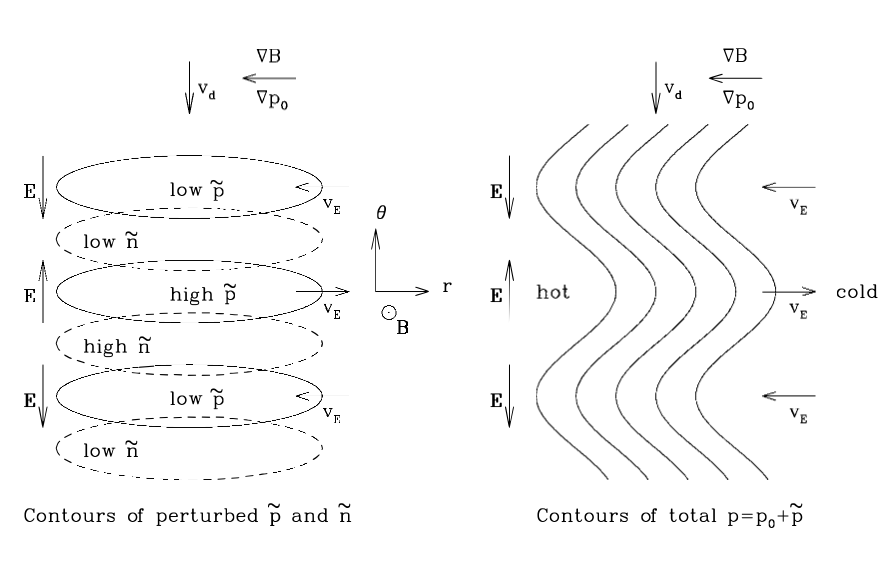
\includegraphics[scale=.7]{Images/ITG_Instability_Cropped.pdf}
         \caption{Simple picture of ITG instability \cite{Beer}.}
      \end{figure}
   \end{frame}

   \begin{frame}{ETG Simulation in GENE}
      \begin{columns}
      \column{0.6\textwidth}
         \begin{figure}
            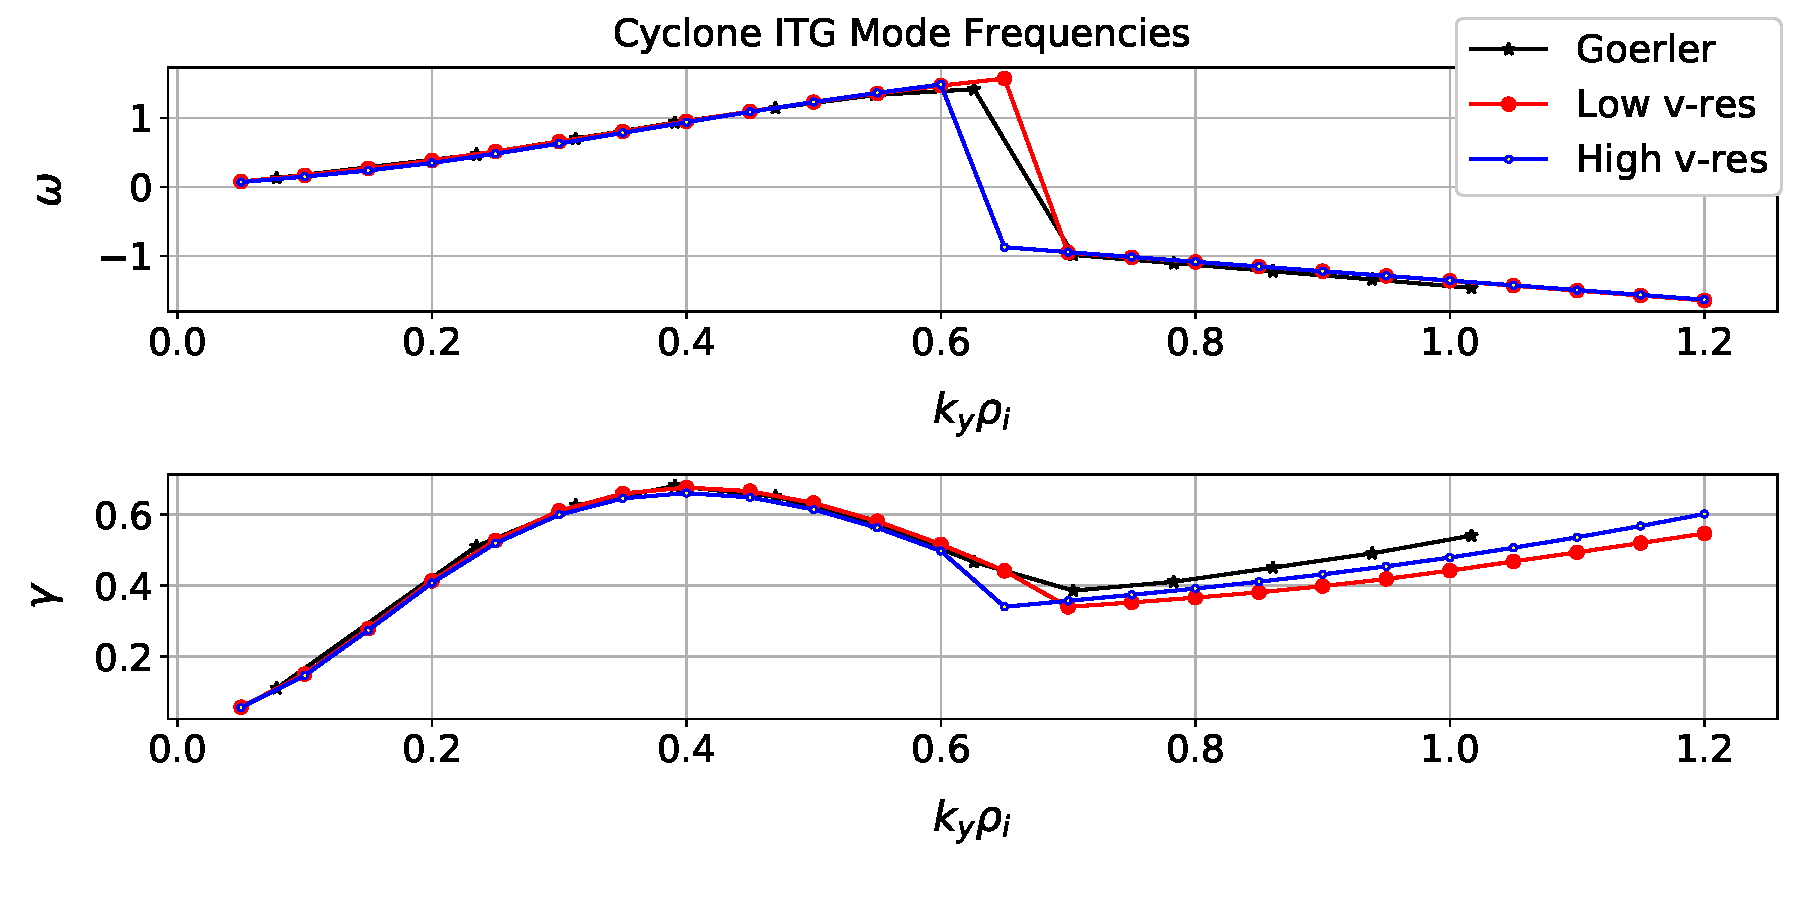
\includegraphics[width=.8\textwidth, height=.35\textheight]{Images/LinearITG_KinEl_GrowthRates.pdf}
            \\
            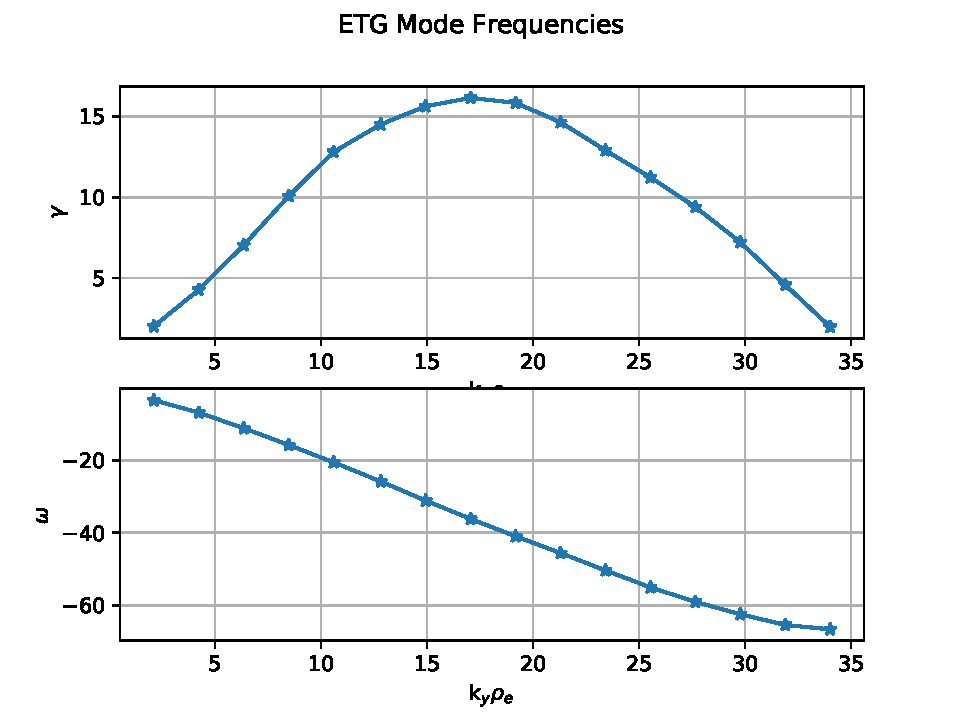
\includegraphics[width=.8\textwidth, height=.45\textheight]{Images/GrowthRates_ETG.pdf}
         \end{figure}
      \column{0.4\textwidth}
         \begin{itemize}
            \item Successful reproduction of G\"{o}rler benchmark with kinetic ions and electrons \cite{Gorler}.
            \vspace{10mm}
            \item Conversion of ITG to ETG flux-tube case prior to running non-linear simulations.
         \end{itemize}
      \end{columns}
   \end{frame}

   \begin{frame}{ETG "Streamers" in GENE}
      \begin{columns}
      \column{0.5\textwidth}
         \begin{figure}
            \hspace*{-.3cm}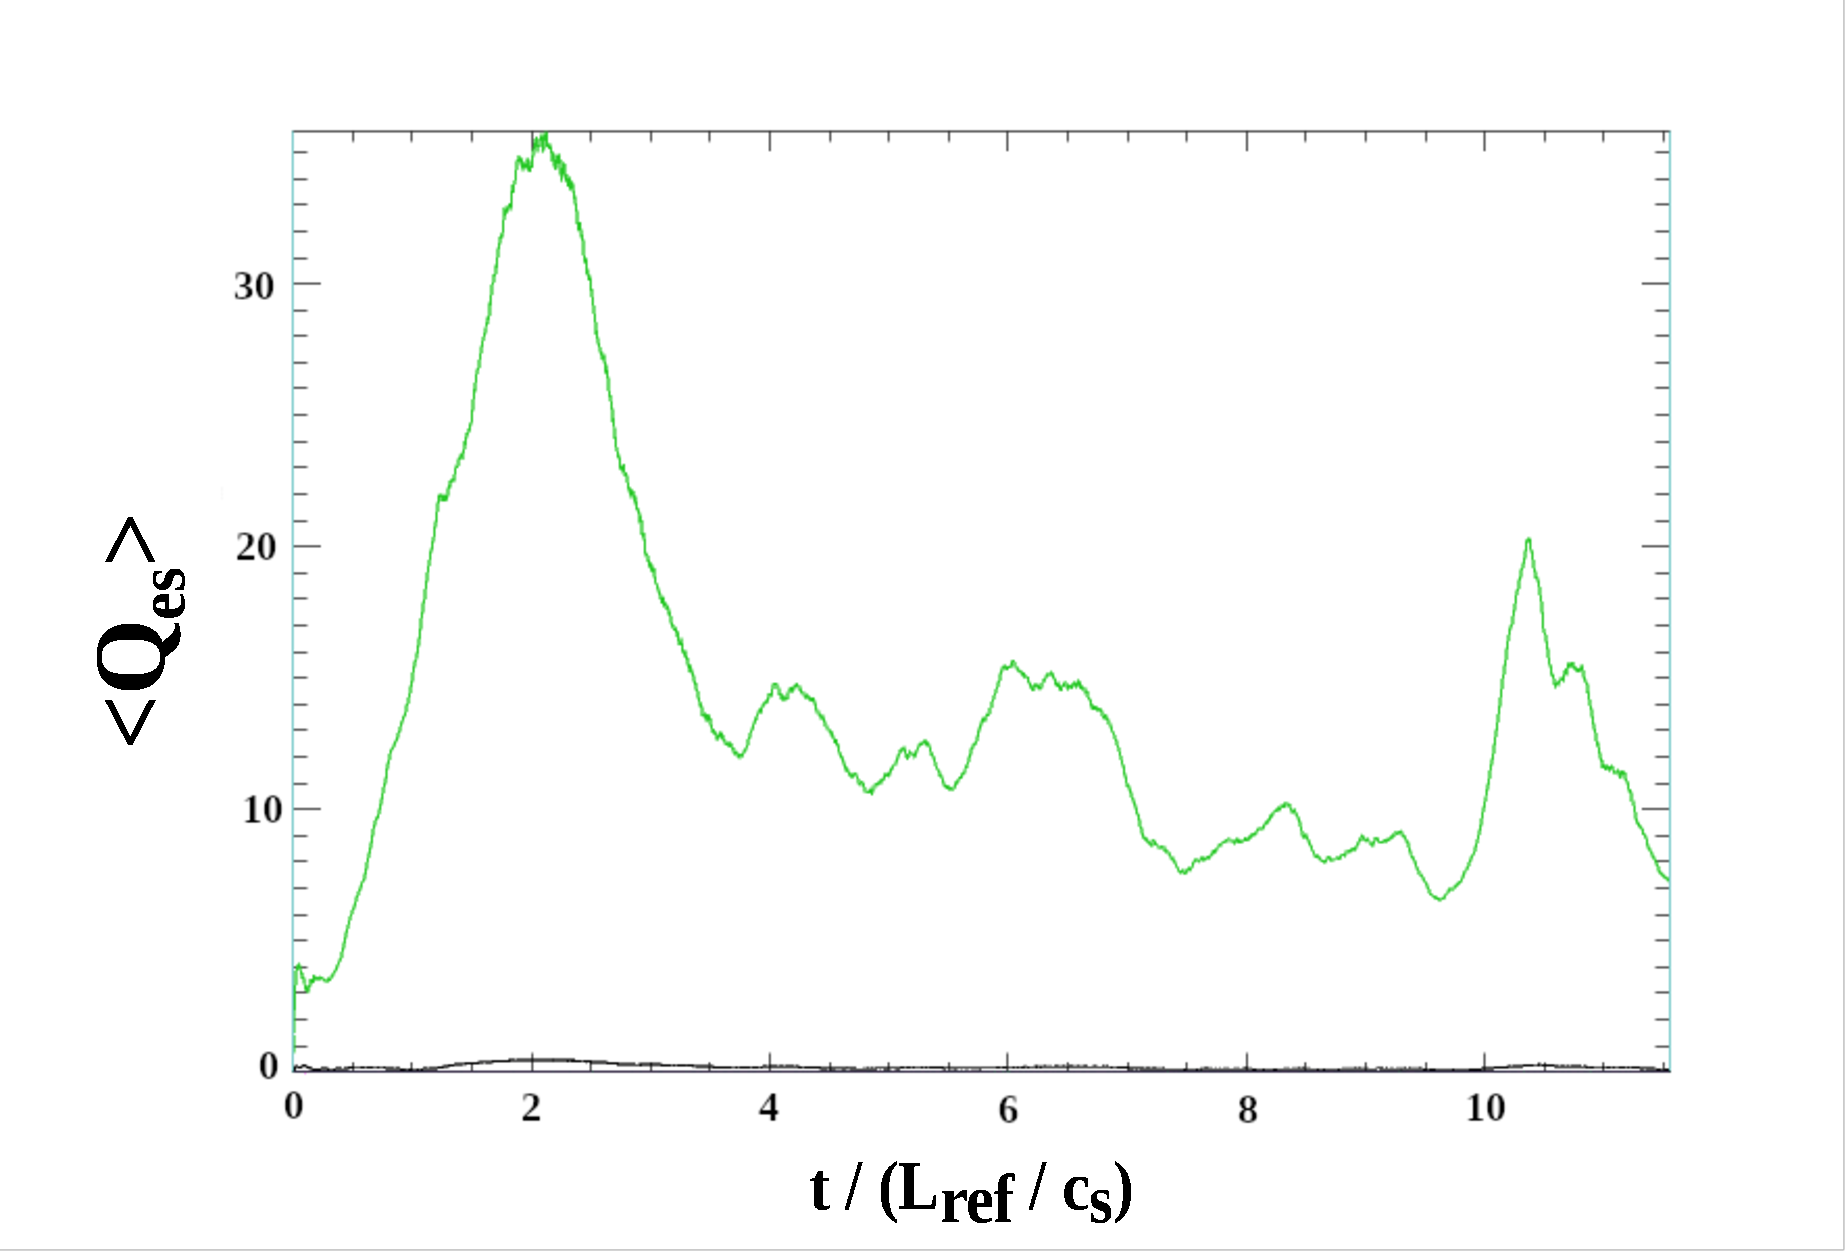
\includegraphics[scale=.3]{Images/etgHeatFlux.pdf}
            \\
            \hspace*{-.3cm}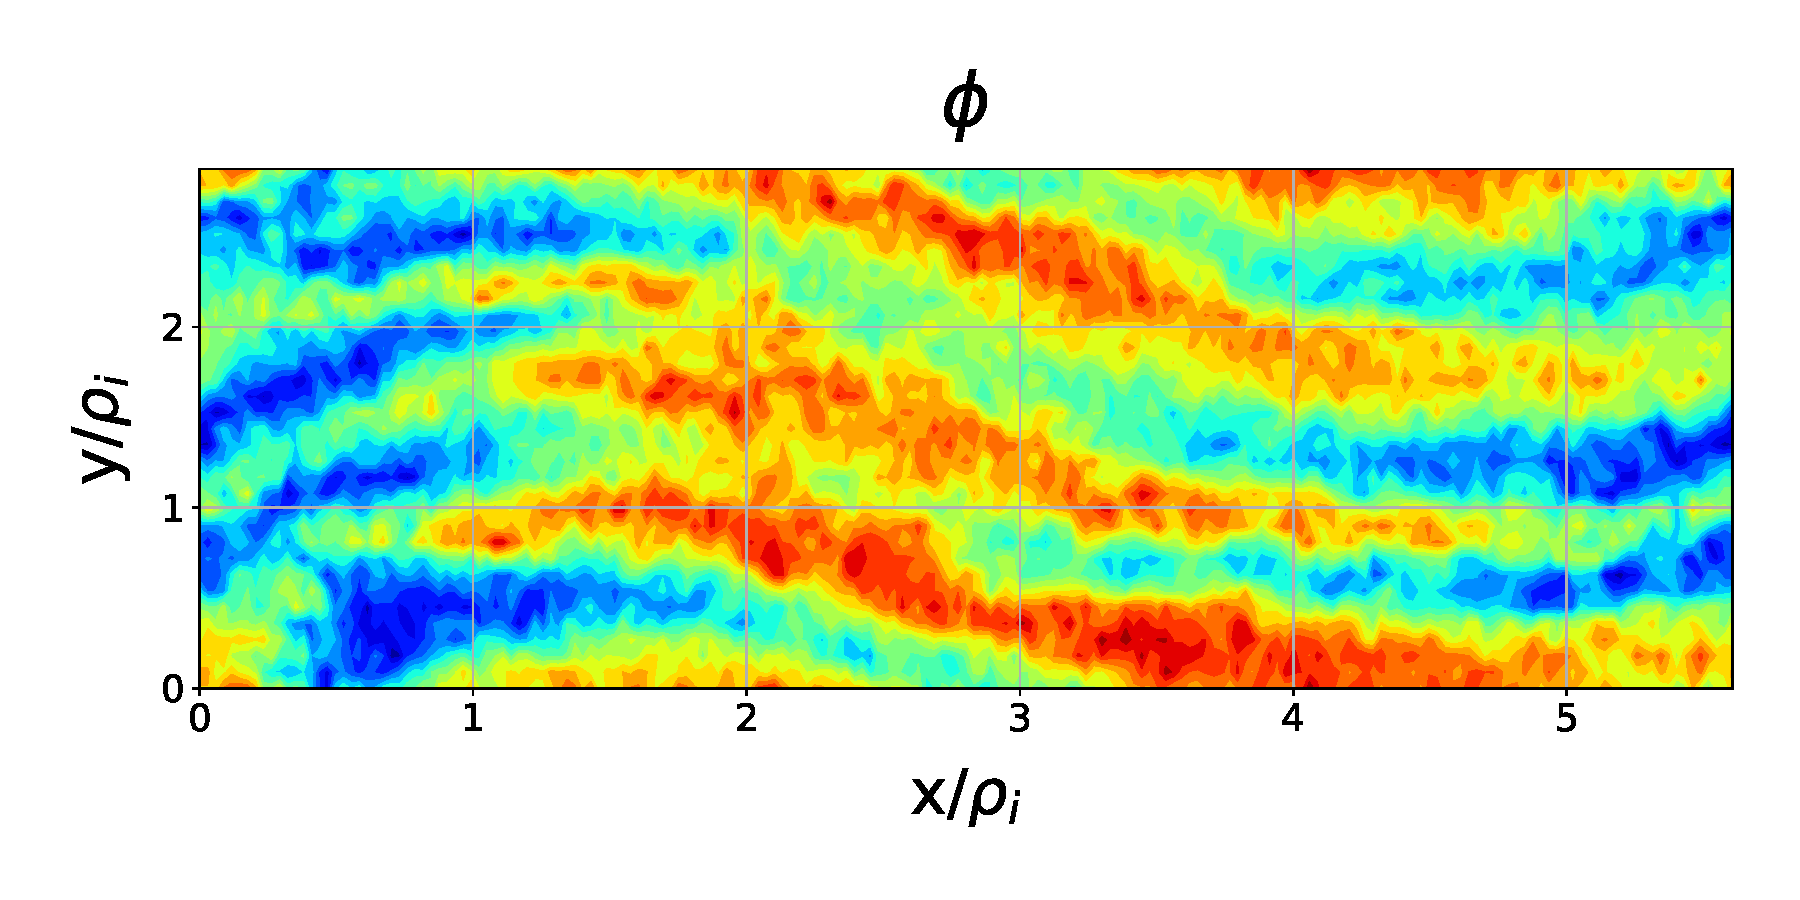
\includegraphics[scale=.2]{Images/genePhiETG_sat2.pdf}
         \end{figure}
      \column{0.5\textwidth}
         \begin{itemize}
            \item ETG turbulence in toroidal gyrokinetic simulations is associated with radially elongated "streamers".
            \vspace{5mm}
            \item Multiscale turbulence simulations have shown that streamers dominate electron heat flux and lead
            to experimental tokamak heat flux values \cite{Howard}.
         \end{itemize}
      \end{columns}
   \end{frame}

   \section{Hasegawa-Mima Fluid Model}

   \begin{frame}{Hasegawa-Mima Fluid ETG Model}
      \begin{itemize}
         \item Partial differential equation derived from fluid continuity and momentum equations.
         \item Approximations made that are useful to describing  turbulence in tokamak plasmas.
         \begin{itemize}
            \item Cyclotron motion periods much smaller than time scales that quantities of interest change on ($B$,$\Phi$,$n$).
            \item Long length scales along $\hat{b}$-direction - $k_{\parallel}/k_{\perp}\equiv\epsilon\ll1$.
            \item Quasi-neutrality of particle densities is enforced.
            \item Adiabatic ions.
            \item Isothermal equation of state, with $\delta P_e = \delta n_eT_e\;(\delta T_e=0)$.
         \end{itemize}
         \item Shown to cause isotropic behavior for long wavelength modes as well as an inverse energy-cascade \cite{Hasegawa}.
      \end{itemize}
   \end{frame}

   \begin{frame}{Hasegawa-Mima Equations}
      \quad We start with the fluid continuity and momentum equations with $\tau = T_e/T_i$, where we have already taken the approximations discussed
   on the previous slide:
      \begin{equation}
         \frac{\partial n_e}{\partial t} + \nabla\cdot\left(n_e\vec{v}_e\right) = 0,
      \end{equation}
      %
      \begin{equation}
            m_e\frac{d\vec{v}_e}{dt} = \left(1+\tau\right)e\nabla\delta\Phi - \frac{e}{c}\vec{v}_e\times\vec{B}-\frac{\nabla P_e}{n_e}\;.
      \end{equation}
      %
      \quad Then $\vec{v}_e$ is solved for using (2) and plugged into (1), dropping terms higher order than $\epsilon$
      to get a final PDE describing the evolution of $\delta\Phi$. The derivation is carried out in Appendix A.
   \end{frame}

   \begin{frame}{Hasegawa-Mima Equations}
      \quad Taking a standard electron dynamic normalization,
      \begin{equation}
      \begin{aligned}
         \Phi    = \frac{e\delta\Phi}{T_i},&\; -\frac{1}{r_n}=\frac{\partial_x n_e}{n_e},\; -\frac{1}{r_t}=\frac{\partial_x T_e}{T_e},\; \eta_e=\frac{r_n}{r_t},\; \\
         \rho_e &= \sqrt{\frac{\tau m_e}{m_i}}\rho_i,\; \vec{x} = \frac{\vec{x}}{\rho_e},\; t=\frac{\rho_e}{r_n}\omega_{ce}t,
      \end{aligned}
      \end{equation}
   and plugging into (10) gives the form of the H-M ETG model,
      \begin{equation}
      \begin{aligned}
         &-(1-\frac{1+\tau}{2\tau}\nabla_{\perp}^2)\partial_t\Phi + \frac{1+\tau}{2\tau}\frac{r_n^2}{\rho_e^2}\partial_t^{-1}\nabla_{\parallel}^2\Phi
          + \frac{(1+\tau)(1+\eta_e)}{4\tau}\partial_y\nabla_{\perp}^2\Phi \\
         &+ \frac{1+\eta_e}{2\tau}\partial_y\Phi + \frac{(1+\tau)^2}{\tau^2}\frac{r_n}{4\rho_e}(\hat{b}\times\nabla_{\perp}\Phi\cdot\nabla_{\perp})\nabla_{\perp}^2\Phi = 0\;.
      \end{aligned}
      \end{equation}
   \end{frame}

   \begin{frame}{Hasegawa-Mima Equations}
      \quad We drop the higher order parallel gradient term and simplify the bracketed expression for a 2-D slab geometry to find the final
   form,
      \begin{equation}
      \begin{aligned}
         \partial_t[\Phi-\frac{1+\tau}{2\tau}\zeta] &= \frac{(1+\tau)(1+\eta_e)}{4\tau}\zeta_y + \frac{1+\eta_e}{2\tau}\Phi_y \\
                                                    &+ \frac{(1+\tau)^2}{\tau}\frac{r_n}{4\rho_e}[\Phi_x\zeta_y-\zeta_x\Phi_y],
      \end{aligned}
      \end{equation}
   where $\zeta = \nabla^2\Phi$ and $x,y$ subscripts denote partial derivatives. The non-linear terms lead to rotation in k-space and eventually isotropization.
   \end{frame}

   \begin{frame}{Pseudo-Spectral Solver}
      \begin{itemize}
         \item Equation (6) is solved numerically using the pseudo-spectral method.
            \begin{itemize}
               \item Fourier transform the equation and get $\zeta=-(k_x^2 + k_y^2)\Phi$.
               \item Inverse Fourier transform $\zeta_{x,y}$ and $\Phi_{x,y}$ back into real space.
               \item Calculate the non-linear products between $\zeta$ and $\Phi$ in real space and then Fourier transform the
               products so they can be added to the other terms in Fourier space.
               \item Time advance $\Phi$ discretely.
            \end{itemize}
         \vspace{5mm}
         \item Time advancement is done using the $4^{th}$ order Runge-Kutta method.
         \vspace{5mm}
         \item The pseudo-spectral method requires de-aliasing of modes due to non-linear terms. This is explored in Appendix B.
      \end{itemize}
   \end{frame}

   \begin{frame}{ETG H-M Results}
      %
      \begin{columns}
         \column{0.7\textwidth}
            \begin{figure}
               \vspace*{-.5cm}
               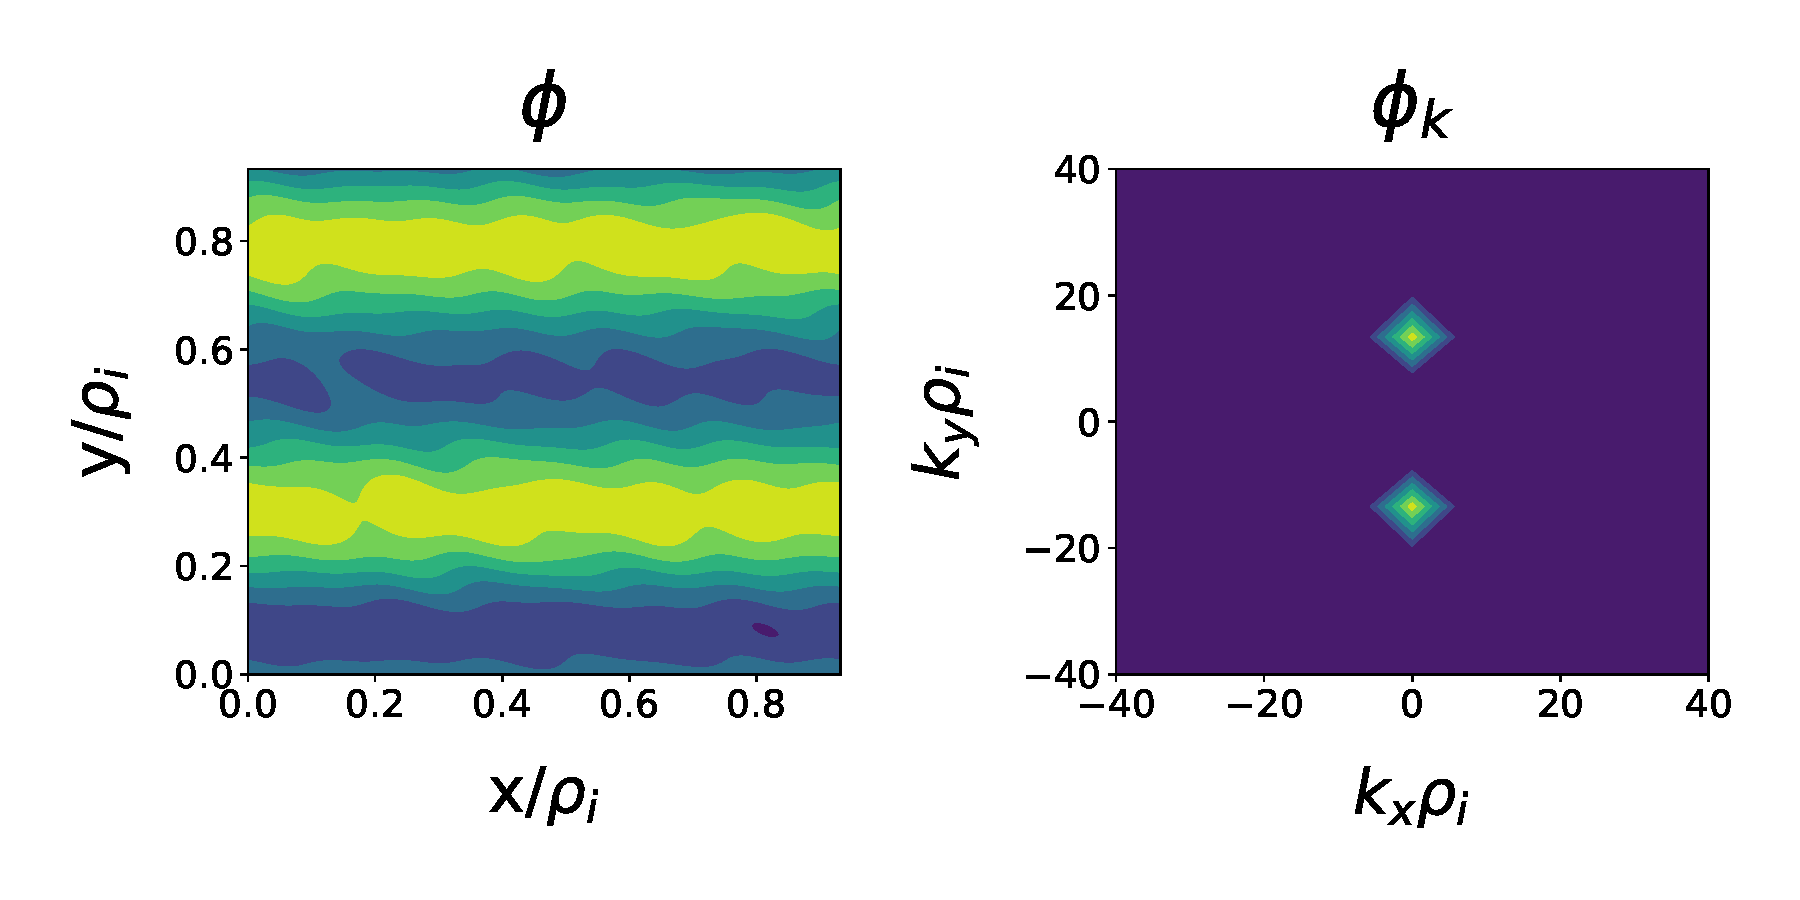
\includegraphics[height=.43\textheight, width=\textwidth]{Images/hmPhiETG_init.pdf}
               \\
               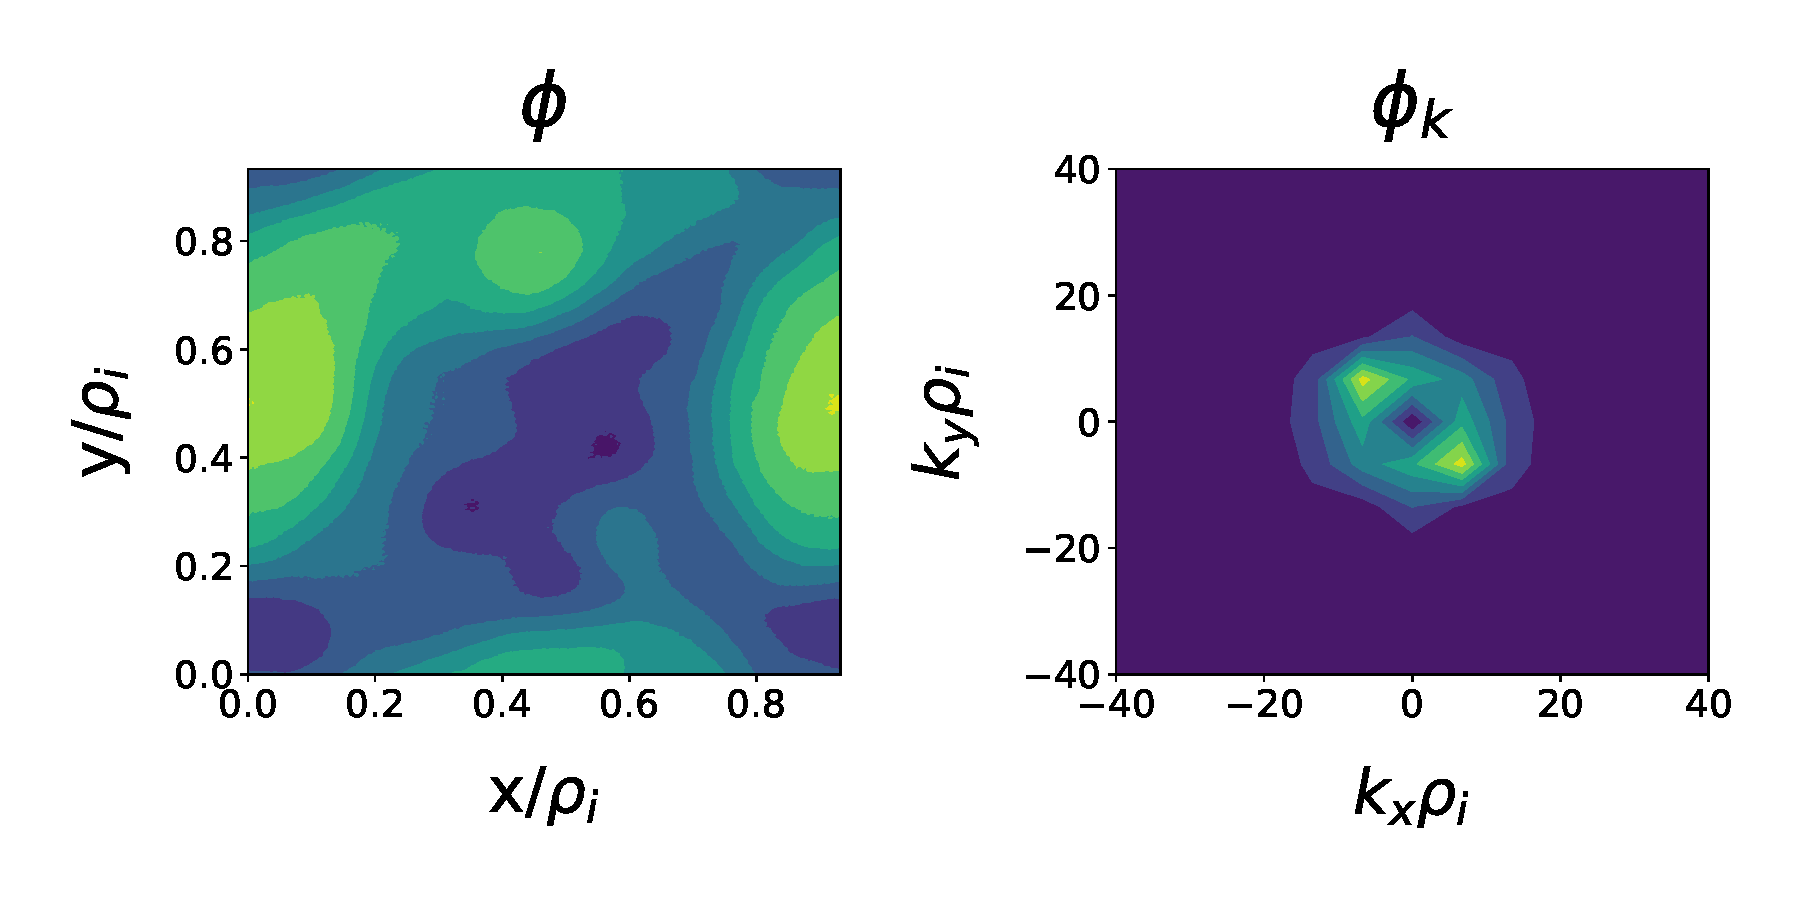
\includegraphics[height=.43\textheight, width=\textwidth]{Images/hmPhiETG_iso.pdf}
            \end{figure}
         \column{0.3\textwidth}
            \begin{itemize}
               \vspace*{-1cm}
               \item Results of H-M code. Initial condition (above) isotropizes at late time (below).
               \item Parameters:
                  \begin{itemize}
                     \item $\tau=1$
                     \item $\eta_e=3$
                     \item $r_n/\rho_i=500$
                  \end{itemize}
            \end{itemize}
      \end{columns}
   \end{frame}

   \begin{frame}{GENE ETG Streamer Test}
      \begin{columns}
         \column{0.7\textwidth}
            \begin{figure}
               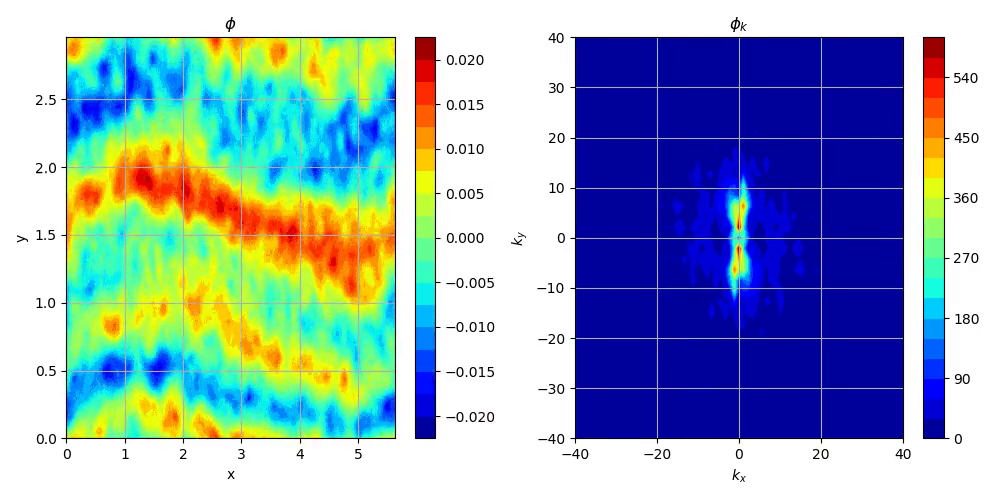
\includegraphics[height=.4\textheight,width=\textwidth]{Images/hmETG_geneInit.png}
               \\
               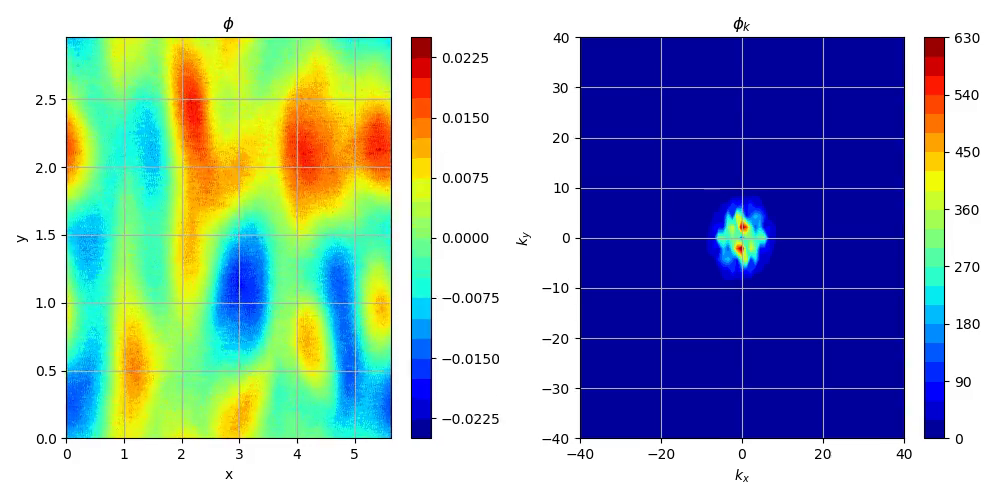
\includegraphics[height=.4\textheight,width=\textwidth]{Images/hmETG_geneIso.png}
            \end{figure}
         \column{0.3\textwidth}
            \begin{itemize}
               \item Test of GENE saturated ETG results into H-M code. Initial condition (above) isotropizes at late time (below).
               \item Inverse energy cascade observed as well.
            \end{itemize}
      \end{columns}
   \end{frame}

   \section{Zonal Flow Excitation}

   \begin{frame}{Zonal Flow Excitation}
      \begin{columns}
         \column{0.6\textwidth}
            \begin{figure}
               \vspace*{-.6cm}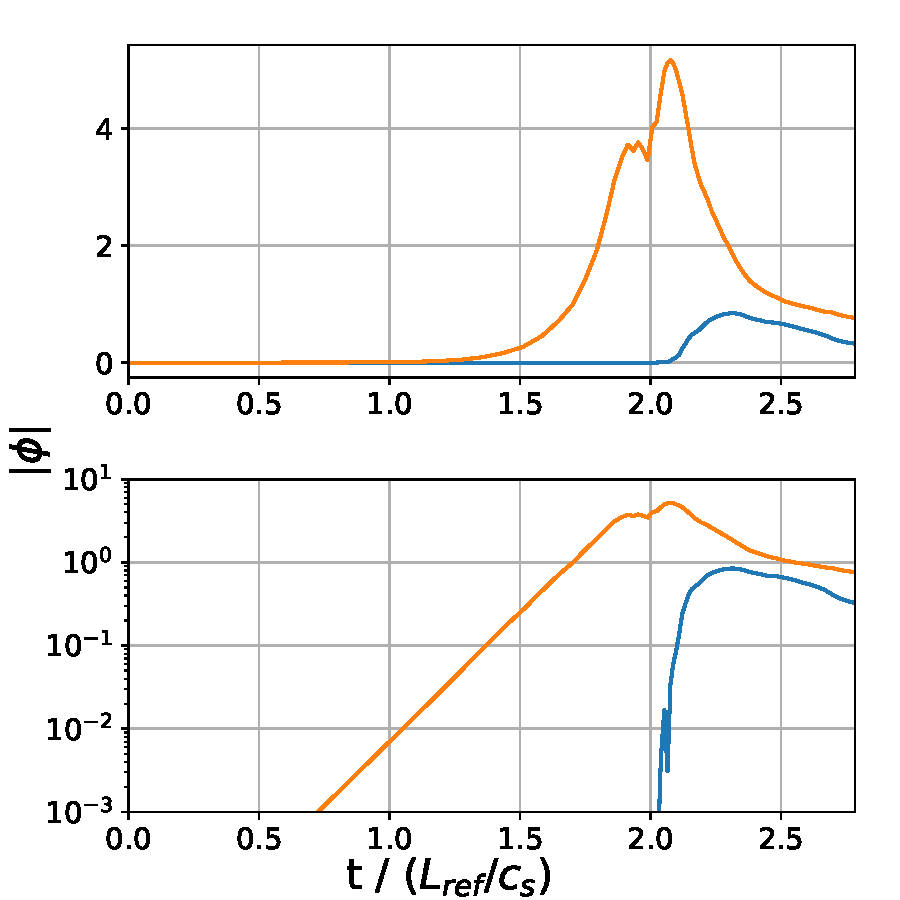
\includegraphics[scale=.45]{Images/zonalFlow.pdf}
            \end{figure}
         \column{0.4\textwidth}
            \vspace*{-.5cm}
            \begin{itemize}
               \item Zonal flow can be spontaneously excited by intermediate-scale ETG turbulence in tokamak geometries - 
               $k_{\perp}\rho_e \ll 1 \ll k_{\perp}\rho_i$.
               \item Plan to carry out large-scale ETG simulations with GENE to compare to theory of zonal flow excitation by ETG modes.
            \end{itemize}
      \end{columns}
   \end{frame}

   \begin{frame}{Four-Wave Weak Turbulence Model}
      \vspace*{-1cm}
      \begin{equation}
      \begin{aligned}
         (\partial_{t}+\gamma_{z}(1+d_{z}k_{z}^{2}\rho_{e}^{2}))\chi_{z}A_{z}\nonumber &=
         \sqrt{\pi/2} W k_{z}^{3}\rho_{e}^{3}(A_{+}A^{*}_{0}a_{n}^{*}-A^{*}_{-}A_{0}a_{n}),         \\
         [\partial_{t}+ i\Delta-\gamma_{s}]A_{+}&=-W k_{z}\rho_{e}A_{z}A_{0}/\sqrt{2\pi},           \\
         [\partial_{t}+ i\Delta-\gamma_{s}]A_{-}&=W k_{z}\rho_{e}A^{*}_{z}A_{0}/\sqrt{2\pi},        \\
         [\partial_{t}-\gamma_{n}]A_{0}&=-W k_{z}\rho_{e}( A_{z}A_{-}-A^{*}_{z}A_{+})/\sqrt{2\pi},  \\
         (\partial_{t}-2\gamma_{n})|A_{0}|^{2}&=(2\gamma_{s}-\partial_{t})(|A_{+}|^{2}+|A_{-}|^{2}) \\
      \end{aligned}
      \end{equation}
      \begin{columns}
      \hspace{1cm}
      \column{.5\textwidth}
         \begin{itemize}
            \item $A_z\equiv$ Zonal Flow Amp.
            \item $A_{\pm}\equiv$ Sideband Amp.'s
            \item $A_0\equiv$ ETG Pump Wave
            \item $a_n\equiv$ Parallel coupling fn.
         \end{itemize}
      \column{.4\textwidth}
         \begin{itemize}
            \item $W\equiv$ Bandwidth
            \item $\gamma_{z,n,s}\equiv$ Growth rates
            \item $\chi_z\equiv$ Susceptibility
            \item $k_z\equiv$ radial k
         \end{itemize}
      \end{columns}
   \end{frame}

   \section*{References}
      \begin{frame}{References}
          \begin{thebibliography}{0}
             \bibitem{Horton} W. Horton, Rev. Mod. Phys. \textbf{71}, 735 (1999).
             \bibitem{Beer} M. A. Beer, \textit{Ph.D. Thesis - Gyrofluid Models of Turbulent Transport in Tokamaks}, Princeton University (1994).
             \bibitem{Gorler} T. G\"{o}rler \textit{et al}, Phys. Plasmas \textbf{23}, 072503 (2016).
             \bibitem{Howard} N.T. Howard \textit{et al} 2016 Nucl. Fusion \textbf{56} 014004
             \bibitem{Hasegawa} A. Hasegawa and Y. Kodama, Phys. Rev. Lett. \textbf{41}, 1470 (1978).
          \end{thebibliography}
      \end{frame}

   \section*{Appendix}

   \begin{frame}{Appendix A: H-M Fluid Model}
      \quad We break up (2) into parallel and perpendicular components by taking a dot product with $\hat{b}$ to find,
      \begin{equation}
         \frac{d\vec{v}_{e,\parallel}}{dt} = (1+\tau)\frac{e}{m_e}\partial_t^{-1}\nabla_{\parallel}\delta\Phi \Rightarrow v_{\parallel}
            \simeq (1+\tau)\frac{k_{\parallel}e\delta\Phi}{m_e\omega},
      \end{equation}
      %
      \begin{equation}
         \frac{d\vec{v}_{e,\perp}}{dt} = (1+\tau)\frac{e}{m_e}\nabla_{\perp}\delta\Phi - \omega_{c,e}\vec{v}_{e,\perp}-\frac{\hat{b}\times\nabla P_e}{m_en_e}\;.
      \end{equation}
   \end{frame}

   \begin{frame}{Appendix A: H-M Fluid Model}
      \quad Then we can split up $\vec{v}_e$ by ordering
      \begin{equation}
      \begin{aligned}
         \vec{v}_{e,0} &= \vec{v}_{\parallel} + \vec{v}_{\perp,0} = \vec{v}_{\parallel} + \left(1 + \tau\right)\vec{v}_E + \vec{v}_D,  \\
         \vec{v}_{e,1} &= \vec{v}_{\perp,1} = -\frac{1}{\omega_{c,e}}(\partial_t+\vec{v}_{e,0}\cdot\nabla)(\hat{b}\times\vec{v}_{e,0}) \\
                       &\simeq \frac{e(1+\tau)}{m_e\omega_{c,e}^2}\partial_t\nabla_{\perp}\delta\Phi - [\frac{\vec{b}\times\nabla P_e}{n_e}\cdot\nabla_{\perp}]
                               \frac{e(1+\tau)}{m_e^2\omega_{c,e}^3}\nabla_{\perp}\delta\Phi \\
                       &+      \frac{e^2(1+\tau)^2}{m_e^2\omega_{c,e}^3}[\hat{b}\times\nabla_{\perp}\delta\Phi\cdot\nabla_{\perp}]\nabla_{\perp}\delta\Phi\;.
      \end{aligned}
      \end{equation}
   \end{frame}

   \begin{frame}{Appendix A: H-M Fluid Model}
      \quad Now, with incompressibility to lowest order, $\nabla\cdot\vec{v}_{e,0,\perp}=0$ and so (1) becomes,
      \begin{equation}
         \partial_t\delta n_e+n_e\nabla\cdot(v_{\parallel} + \vec{v}_{e,1}) + \nabla\delta n_e\cdot\vec{v}_D+(1+\tau)\delta n_e\cdot\vec{v}_E = 0,
      \end{equation}
      and plugging in $\delta n_e=\delta n_i$, we find that to order $\epsilon$,
      \vspace{-2mm}
      \begin{equation}
      \begin{aligned}
         &-n_e\partial_t\frac{e\delta\Phi}{T_i} + n_e(1+\tau)\frac{e}{m_e}\partial_t^{-1}\nabla_{\parallel}^2\delta\Phi
         + \frac{en_e(1+\tau)}{m_e\omega_{c,e}^2}\partial_t\nabla_{\perp}^2\delta\Phi \\
         &- \frac{e(1+\tau)}{m_e^2\omega_{c,e}^3}[\hat{b}\times\nabla P_e\cdot\nabla_{\perp}]\nabla_{\perp}^2\delta\Phi
         + \frac{e^2n_e(1+\tau)^2}{m_e^2\omega_{c,e}^3}[\hat{b}\times\nabla_{\perp}\delta\Phi\cdot\nabla_{\perp}]\nabla_{\perp}^2\delta\Phi \\
         &+ \nabla_{\perp}\frac{e\delta\Phi}{T_i}\cdot\frac{\hat{b}\times\nabla P_e}{m_e\omega_{c,e}} + \frac{e(1+\tau)}{m_e\omega_{c,e}}\nabla n_e\cdot\hat{b}\times\nabla\Phi = 0\;.
      \end{aligned}
      \end{equation}
   \end{frame}

   \begin{frame}{Appendix B: Pseudo-Spectral De-Aliasing}
   \end{frame}

\end{document}